\documentclass[border=3pt]{standalone}
% Preâmbulo compartilhado pelos diagramas TikZ da aula 7 (Filtros Não Paramétricos)
\usepackage[T1]{fontenc}
\usepackage[utf8]{inputenc}
\usepackage{lmodern}
\usepackage{amsmath}
\usepackage{xcolor}
\usepackage{tikz}
\usetikzlibrary{arrows.meta,angles,quotes,decorations.pathmorphing,calc,
                positioning,shapes.geometric,shapes.misc,backgrounds,fit,
                math}

% Paleta (mesma dos SVGs originais)
\definecolor{dblue}{HTML}{2A5B8C}
\definecolor{dorange}{HTML}{B3541E}
\definecolor{dgreen}{HTML}{4A7C59}
\definecolor{dred}{HTML}{9C4B4B}
\definecolor{dcream}{HTML}{F4F1EA}
\definecolor{dshade}{HTML}{DDD7C9}

% Função gaussiana (não normalizada por padrão de escala visual)
\pgfmathdeclarefunction{gauss}{3}{%
  \pgfmathparse{1/(#3*sqrt(2*pi))*exp(-((#1-#2)^2)/(2*#3^2))}%
}

% Estilos comuns (prefixo d... para não colidir com chaves internas do pgf)
\tikzset{
  >={Stealth[length=2mm]},
  dguide/.style={gray!55, dashed, line width=0.4pt},
  daxis/.style={gray!60, line width=0.7pt, ->},
  dbody/.style={fill=black!3, draw=black!80, line width=1pt},
  dacc/.style={draw=dblue, line width=1pt},
  dlbl/.style={black!55, font=\small},
  dsub/.style={black!45, font=\footnotesize},
  dstate/.style={circle, draw=black!80, fill=dcream, line width=1pt,
                 minimum size=17mm, font=\large, inner sep=1pt},
  dobs/.style={circle, draw=black!80, fill=dshade, line width=1pt,
               minimum size=14mm, font=\large, inner sep=1pt},
  dbox/.style={rounded corners=2pt, draw=black!80, fill=dcream, line width=1pt,
               align=center, inner sep=6pt},
  dop/.style={circle, draw=black!80, fill=white, line width=1pt,
              minimum size=6mm, inner sep=0pt, font=\small},
  dtrans/.style={->, dblue, line width=1pt},
  dmeas/.style={->, dorange, line width=1pt},
  dcurve/.style={line width=1pt, dblue},
  dcurveb/.style={line width=1.4pt, dorange},
}

\begin{document}
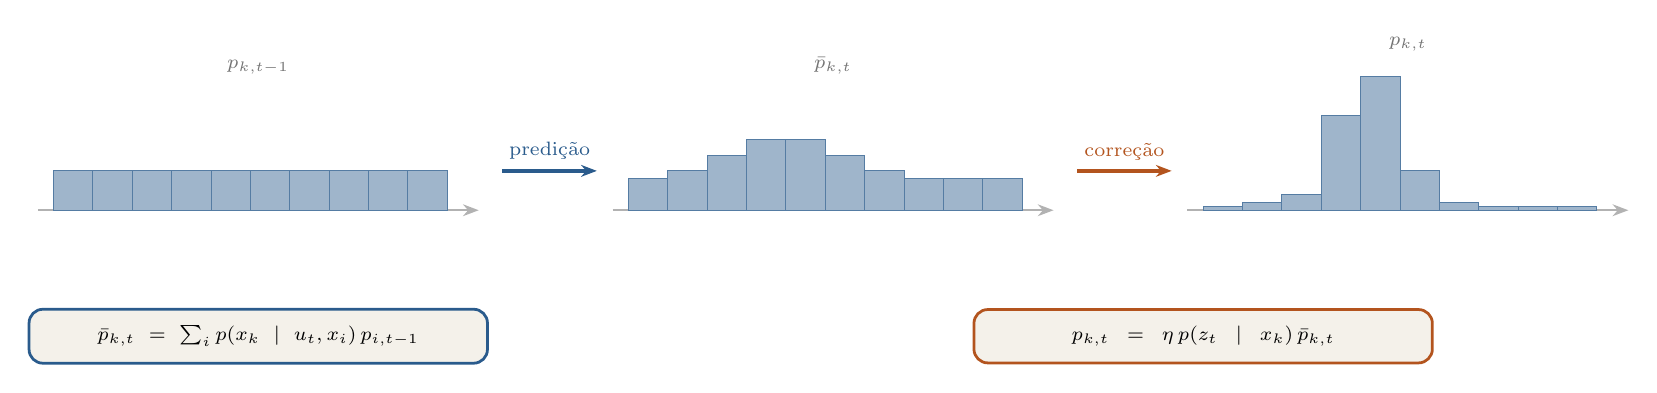
\begin{tikzpicture}[x=1cm,y=1cm]
  \newcommand{\barras}[3]{\draw[daxis] (#1,#2) -- (#1+5.6,#2); \foreach \h [count=\i] in {#3} { \fill[dblue!45, draw=dblue!80, line width=0.3pt] ({#1+0.2+(\i-1)*0.5},#2) rectangle ({#1+0.2+\i*0.5},{#2+\h}); }}
  \barras{0}{0}{0.5,0.5,0.5,0.5,0.5,0.5,0.5,0.5,0.5,0.5}
  \node[dlbl, font=\scriptsize, anchor=south] at (2.8,1.6) {$p_{k,t-1}$};
  \draw[dtrans, line width=1.4pt] (5.9,0.5) -- (7.1,0.5) node[midway, above, font=\scriptsize] {predição};
  \barras{7.3}{0}{0.4,0.5,0.7,0.9,0.9,0.7,0.5,0.4,0.4,0.4}
  \node[dlbl, font=\scriptsize, anchor=south] at (10.1,1.6) {$\bar p_{k,t}$};
  \draw[dmeas, line width=1.4pt] (13.2,0.5) -- (14.4,0.5) node[midway, above, font=\scriptsize] {correção};
  \barras{14.6}{0}{0.05,0.1,0.2,1.2,1.7,0.5,0.1,0.05,0.05,0.05}
  \node[dlbl, font=\scriptsize, anchor=south] at (17.4,1.9) {$p_{k,t}$};
  \node[dbox, rounded corners=5pt, text width=5.4cm, font=\scriptsize, draw=dblue] at (2.8,-1.6) {$\bar p_{k,t}=\sum_i p(x_k\mid u_t,x_i)\,p_{i,t-1}$};
  \node[dbox, rounded corners=5pt, text width=5.4cm, font=\scriptsize, draw=dorange] at (14.8,-1.6) {$p_{k,t}=\eta\,p(z_t\mid x_k)\,\bar p_{k,t}$};
\end{tikzpicture}
\end{document}
